\documentclass[11pt,a4paper]{article}

\usepackage[T1]{fontenc}
\usepackage[utf8]{inputenc}
\usepackage[italian]{babel}
\usepackage{amsmath,amssymb}
\usepackage[a4paper,margin=2.5cm]{geometry}
\usepackage{array}
\usepackage{siunitx}
\usepackage{booktabs}
\usepackage{graphicx}
\usepackage{float}
\usepackage{hyperref}

\hypersetup{hidelinks}
\setlength{\parindent}{0pt}
\setlength{\parskip}{4pt}
\allowdisplaybreaks
\graphicspath{{figure/}}
\sisetup{output-decimal-marker={,}, group-separator={\,}, per-mode=symbol,
         exponent-product=\cdot, range-phrase={\text{--}}}

\newcommand{\uma}{u-a}
\newcommand{\upa}{u+a}
\newcommand{\Ms}{M_{s}}

\title{Gasdinamica -- Svolgimento esercizio 1\\[2pt]
\large Condotto tra serbatoio e ambiente: rimozione del setto e transitorio fino allo stato finale}
\author{}
\date{Prova del 01/01/1975}

\begin{document}
\maketitle

\section*{Traccia}
Un serbatoio di grande capacità è collegato all'ambiente per mezzo di un condotto a sezione costante, chiuso da un
setto posto nella sua metà. Al tempo $t_0$ il setto viene rimosso istantaneamente. Determinare l'evoluzione del
campo di moto nel condotto da tempo $t_0$ fino al completamento del transitorio. Il gas nel serbatoio è aria:
$\gamma=1{,}4$ e $R=287$ (stampato ``KJ/kg K''). Le condizioni iniziali del serbatoio: $P_0=\SI{0.04}{atm}$ e
$T_0=\SI{98}{K}$. Le condizioni ambiente: $p=\SI{1}{atm}$ e $T=\SI{287.7}{K}$.

\begin{figure}[H]
  \centering
  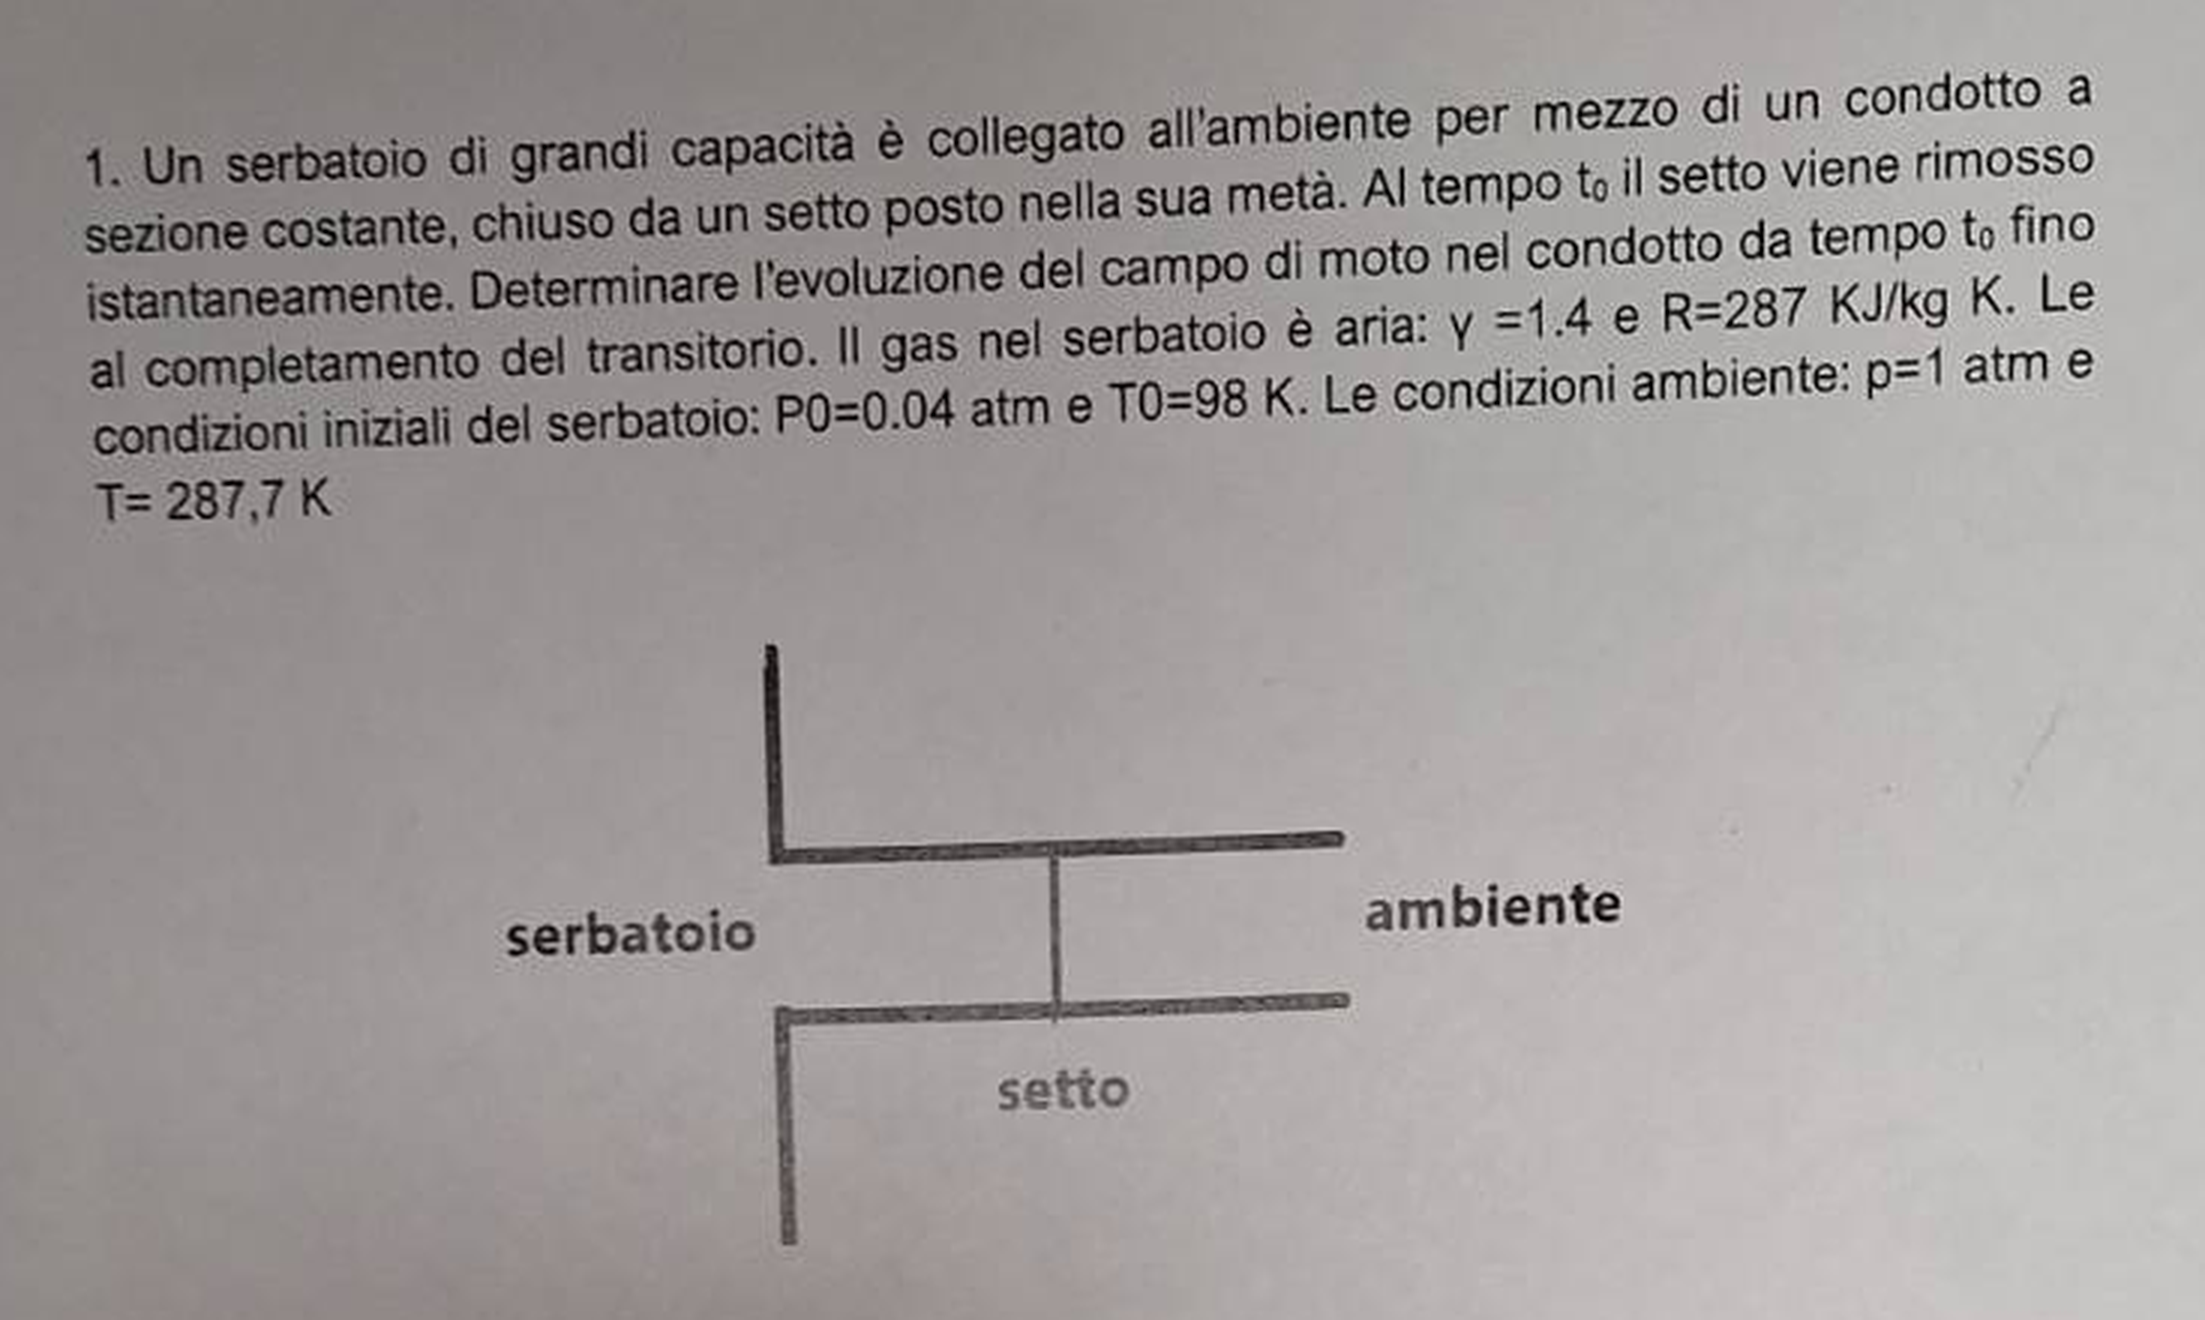
\includegraphics[width=0.62\textwidth]{originale.png}
  \caption{Testo originale dell'esercizio.}
\end{figure}

%==============================================================================
\section{Lettura del testo e dati}
\begin{figure}[H]
  \centering
  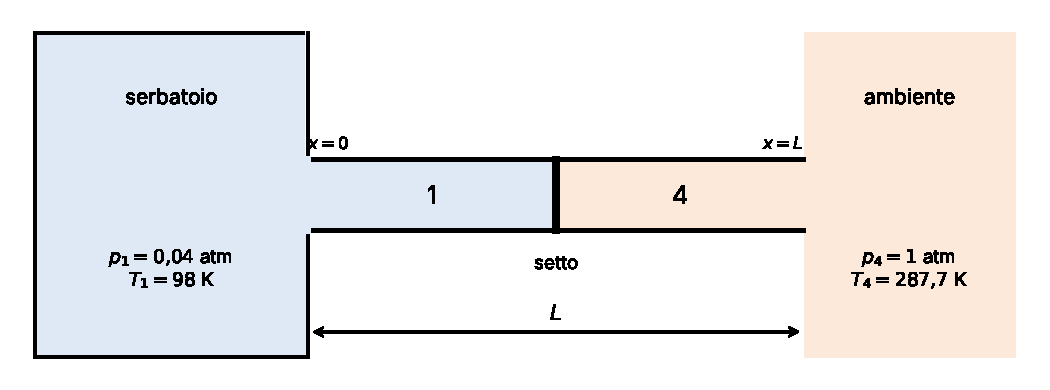
\includegraphics[width=0.78\textwidth]{schema.pdf}
  \caption{Schema: serbatoio in $x=0$, ambiente in $x=L$, setto in $x=L/2$ (non in scala).}
  \label{fig:schema}
\end{figure}
Il condotto è aperto verso il serbatoio e verso l'ambiente; il setto lo divide in due metà. Prima di $t_0$ la
metà sinistra contiene il gas del serbatoio nelle sue condizioni (stato 1), la metà destra l'aria ambiente (stato
4), entrambi in quiete: le condizioni assegnate sono quindi anche quelle totali dei due ``serbatoi'' esterni. Il
testo scrive $R=287$ ``KJ/kg K'': per l'aria il valore è \SI{287}{J/(kg.K)}, e lo leggo così. Entrambi i gas sono
aria. La lunghezza $L$ non è data: uso $x/L$ e il tempo acustico $\tau=L/a_4$, e pongo $t_0=0$.

Il dato che caratterizza il problema è che il serbatoio è a pressione \emph{minore} dell'ambiente: l'aria
ambiente entrerà nel condotto e si scaricherà nel serbatoio. ``Grande capacità'' vuol dire che, durante il
transitorio nel condotto, pressione e temperatura del serbatoio non cambiano; lo stesso vale per l'ambiente.

\begin{table}[H]
  \centering
  \begin{tabular}{lll}
    \toprule
    Grandezza & Valore & Note \\
    \midrule
    $\gamma$, $R$ & \num{1.4}, \SI{287}{J/(kg.K)} & aria ovunque; $\delta=(\gamma-1)/2=\num{0.2}$ \\
    $p_1$, $T_1$ & \SI{0.04}{atm}, \SI{98}{K} & serbatoio e metà sinistra, $u_1=0$ \\
    $a_1=\sqrt{\gamma RT_1}$, $\rho_1$ & \SI{198.4}{m/s}, \SI{0.144}{kg/m^3} & \\
    $p_4$, $T_4$ & \SI{1}{atm}, \SI{287.7}{K} & ambiente e metà destra, $u_4=0$ \\
    $a_4$, $\rho_4$ & \SI{340.0}{m/s}, \SI{1.227}{kg/m^3} & $\tau=L/a_4$ \\
    $p_4/p_1$ & \num{25} & \\
    \bottomrule
  \end{tabular}
  \caption{Dati del problema.}
\end{table}
Si chiede l'evoluzione del campo nel condotto: onde generate, loro riflessioni agli estremi e stato a cui il
condotto tende. Tracce affini nel catalogo: B37-E01 (serbatoio, condotto con setto e condizioni asintotiche) e
B27-E02 (setto fra serbatoio e condotto); l'esempio d'esame del 24/01/2019 (condotto tra serbatoio e ambiente)
ha la stessa struttura di contorni, a parti invertite.

%==============================================================================
\section{Modello e ipotesi}
\begin{itemize}
\item \textbf{Eulero 1D instazionario} nel condotto a sezione costante: diametro piccolo rispetto a $L$, onde
  piane, gas perfetto non viscoso e adiabatico (attrito e scambio termico trascurati).
\item \textbf{Rimozione istantanea} del setto: in $(L/2,0)$ c'è un problema di Riemann.
\item \textbf{Serbatoio e ambiente di grande capacità}: le loro condizioni totali restano costanti durante il
  transitorio. Gli estremi del condotto li tratto come sezioni di raccordo di lunghezza nulla.
\item \textbf{Condizioni al contorno} in numero pari alle caratteristiche entranti. Se il gas \emph{esce} dal
  condotto verso un serbatoio a velocità subsonica impongo la pressione del serbatoio; se esce supersonico non
  impongo nulla. Se il gas \emph{entra} da un serbatoio impongo le sue condizioni totali ($p_0$, $T_0$), non la
  pressione statica.
\item Non assumo a priori un campo omoentropico: urto e contatto possono creare salti di entropia. Lo verifico
  dopo il problema di Riemann (sez.~\ref{sec:calcolo}).
\item Le zone d'interazione a due famiglie non le risolvo punto per punto: ne do la struttura, gli stati
  limite e i fronti. Dove servono stime di tempi tratto le caratteristiche come semirette.
\item Non uso $p_0$ e $h_0$ costanti dentro il condotto: il moto è instazionario.
\end{itemize}

%==============================================================================
\section{Analisi qualitativa}
\textbf{Rimozione del setto.} La pressione è 25 volte maggiore a destra: l'aria ambiente spinge verso sinistra
come un pistone. Nascono un \textbf{urto $\uma$} che corre verso il serbatoio nel gas 1, un \textbf{contatto} e
un'\textbf{espansione centrata $\upa$} che corre verso l'ambiente nel gas 4 (configurazione SCR). I versi sono
coerenti: l'urto spinge il gas nel verso in cui si propaga (verso sinistra), l'espansione lo richiama nel verso
opposto al suo (ancora verso sinistra), quindi $u^*<0$. Con un rapporto di pressione così grande mi aspetto un urto
di intensità finita ($\Ms\approx2$) e un'espansione forte, forse transonica: lo dirà la pendenza della coda.

\textbf{Estremo sinistro.} Quando l'urto arriva in $x=0$ esce nel serbatoio e dietro di lui il gas si scarica nel
serbatoio. Se questo efflusso è supersonico l'uscita non riceve informazione e non nasce nessuna riflessa; se fosse
subsonico la pressione dovrebbe scendere a $p_1$ e si rifletterebbe un'espansione (natura opposta, contorno a
pressione imposta).

\textbf{Estremo destro.} Quando la testa dell'espansione arriva in $x=L$ il gas comincia a entrare dall'ambiente.
L'ingresso impone le condizioni totali: con $p_0$ fissata, la pressione statica all'ingresso scende solo di quanto
serve ad accelerare il gas, cioè resta vicina a $p_4$ finché il Mach è basso. L'ingresso si comporta quindi quasi
come un estremo a pressione costante: l'espansione si riflette come \textbf{compressione $\uma$}, che ricomprime il
gas e lo accelera ancora verso il serbatoio.

\textbf{Fine del transitorio.} A regime il condotto, a sezione costante, porta una corrente stazionaria
isentropica dall'ambiente al serbatoio, quindi uniforme. La pressione del serbatoio, \SI{0.04}{atm}, è molto
minore della pressione critica dell'ambiente ($0{,}528$ atm): il condotto non può adattarsi e la corrente sarà
\textbf{sonica in tutto il condotto}, con getto sottoespanso nel serbatoio. In instazionario si raggiunge $M=1$ in
un condotto a sezione costante, e qui la sezione d'imbocco fa da gola.

%==============================================================================
\section{Topologia del campo}
\label{sec:topologia}
\begin{figure}[H]
  \centering
  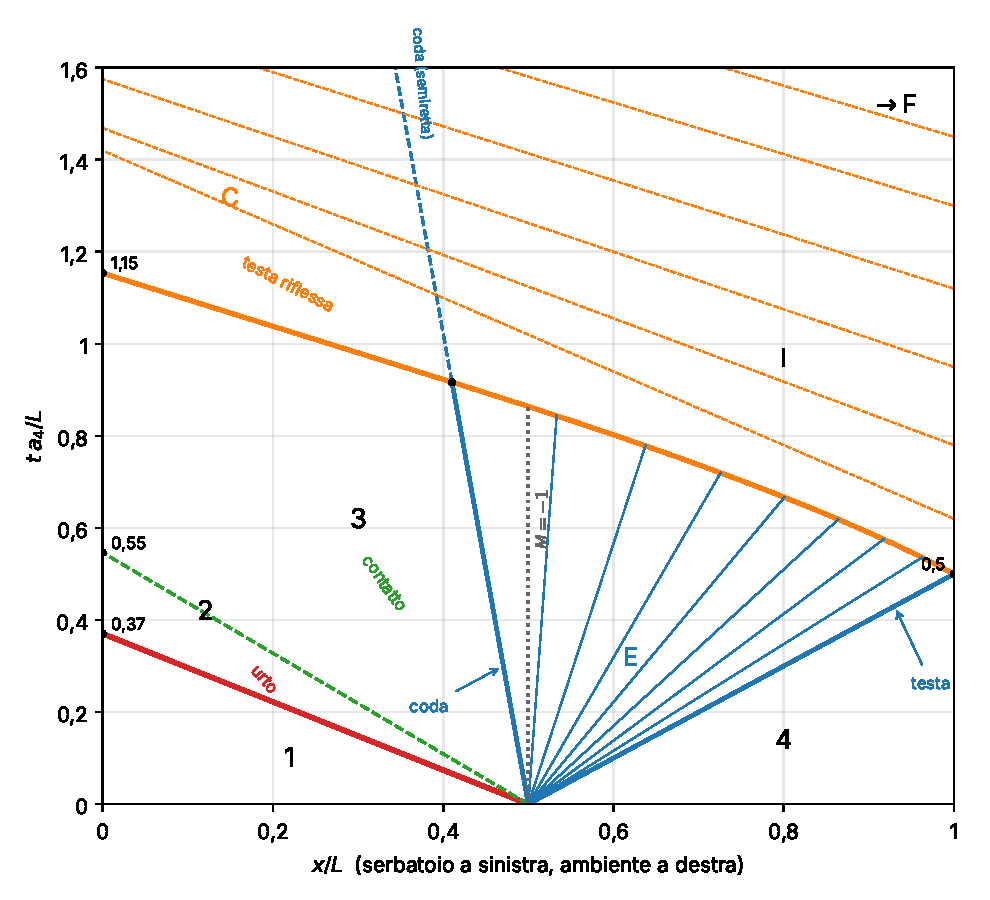
\includegraphics[width=0.72\textwidth]{xt.pdf}
  \caption{Piano $x$--$t$. Urto (rosso), contatto (verde), ventaglio E (blu: testa, coda e raggi), testa della
  compressione riflessa dall'ingresso (arancio, esatta) e alcune compressioni successive (arancio tratteggiato,
  schematiche). Il raggio sonico $x=L/2$ è punteggiato. I tempi in $x=0$ e $x=L$ sono in unità $L/a_4$.}
  \label{fig:xt}
\end{figure}
Regioni del piano $x$--$t$ (fig.~\ref{fig:xt}):
\begin{itemize}
\item \textbf{1}, \textbf{4}: gas iniziali in quiete, uniformi (nessuna famiglia attiva).
\item \textbf{2}, \textbf{3}: stati uniformi dietro l'urto e dietro l'espansione, separati dal contatto.
\item \textbf{E}: espansione centrata $\upa$ con centro in $(L/2,0)$, onda semplice ($R_1=a_4$ uniforme, raggi
  rettilinei). È transonica: il raggio $x=L/2$ è sonico ($M=-1$).
\item \textbf{I}: zona d'interazione a due famiglie fra E e le compressioni $\uma$ riflesse dall'ingresso; qui le
  caratteristiche si curvano.
\item \textbf{C}: compressioni $\uma$ che, uscite da I, attraversano lo stato 3: onda semplice con $R_2=R_{2,3}$
  uniforme, fino alla coda di E (curvata, disegnata come semiretta).
\item \textbf{F}: stato finale sonico, a cui il campo tende per $t\to\infty$.
\end{itemize}
Fronti: l'urto raggiunge $x=0$ a $0{,}37\,\tau$ e il contatto a $0{,}55\,\tau$; la testa di E raggiunge $x=L$ a
$0{,}5\,\tau$; la testa della compressione riflessa attraversa E lungo una curva e lo stato 3 lungo una retta,
fino a $x=0$ a $\approx1{,}15\,\tau$. Nessuna onda risale dall'uscita nel serbatoio. Il diagramma è commentato con i
numeri in sez.~\ref{sec:rappr}.

%==============================================================================
\section{Bilancio equazioni/incognite}
\begin{itemize}
\item \textbf{Riemann SCR}: incognite $\rho_2,u_2,p_2,\rho_3,u_3,p_3$ e la velocità dell'urto $w$ (7). Equazioni:
  3 di Rankine--Hugoniot, 2 dell'espansione ($R_1$ e $s$ costanti), 2 del contatto ($p_2=p_3$, $u_2=u_3$).
\item \textbf{Ingresso} $x=L$, flusso entrante subsonico: entrano le caratteristiche $u$ e $\uma$, esce la $\upa$.
  Tre incognite ($\rho,u,p$) = 2 condizioni ($s=s_4$, $h_0=h_{0,4}$) + 1 compatibilità ($R_2$ dall'interno).
\item \textbf{Uscita} $x=0$, flusso uscente supersonico: tutte e tre le caratteristiche escono, nessuna condizione.
\item \textbf{Stato finale}: tre incognite uniformi = 2 condizioni d'ingresso + condizione sonica (il serbatoio è
  sotto la pressione critica e non può fissare la pressione d'uscita).
\end{itemize}

%==============================================================================
\section{Scorciatoie fisiche}
\begin{itemize}
\item \textbf{Contatto nullo} (risultato del calcolo di Riemann): l'urto porta il gas freddo del serbatoio
  esattamente all'entropia dell'aria ambiente. Dopo il passaggio dell'urto il condotto è omoentropico con $s=s_4$,
  quindi gli invarianti $R_1$, $R_2$ valgono esattamente in tutto il campo successivo, zone d'interazione comprese.
\item \textbf{Uscita supersonica}: il serbatoio non manda informazioni nel condotto, quindi la sua pressione conta
  solo nel problema di Riemann iniziale.
\item \textbf{Stato finale noto senza risolvere il transitorio}: ingresso sonico con le condizioni totali
  dell'ambiente.
\end{itemize}

%==============================================================================
\section{Calcolo}
\label{sec:calcolo}

\subsection*{Problema di Riemann in $(L/2,0)$}
\textbf{Primo tentativo} (isentropico, sulla velocità):
\[
z=\frac{a_4}{a_1}\left(\frac{p_1}{p_4}\right)^{\frac{\gamma-1}{2\gamma}}=\num{1.082},\qquad
u^{(0)}=\frac{z(a_1+\delta u_1)-(a_4-\delta u_4)}{\delta(1+z)}=\SI{-301}{m/s}.
\]
$u^{(0)}<u_1$: a sinistra urto; $u^{(0)}<u_4$: a destra espansione. Con questa velocità
\[
M_{\rm rel,1}=\frac{\gamma+1}{4}\frac{u_1-u}{a_1}+\sqrt{1+\left(\frac{\gamma+1}{4}\frac{u_1-u}{a_1}\right)^2},\quad
p_2=p_1\left[1+\frac{2\gamma}{\gamma+1}\left(M_{\rm rel,1}^2-1\right)\right]=\SI{0.232}{atm},
\]
\[
a_3=a_4+\delta(u-u_4),\qquad p_3=p_4\left(\frac{a_3}{a_4}\right)^{\frac{2\gamma}{\gamma-1}}=\SI{0.256}{atm}.
\]
Lo scarto è del 9\,\%: l'urto non è debole e il tentativo isentropico va corretto. Aggiornando $u$ con la
pendenza delle due curve ($u^{k+1}=u^k-(p_2^k-p_3^k)/(\dot p_2^k-\dot p_3^k)$) già il secondo passo dà
$|p_2-p_3|/p^*<10^{-3}$, cioè fisicamente nullo:
\[
u^*=\SI{-311.0}{m/s},\qquad p^*=\SI{0.243}{atm}.
\]

\textbf{Stato 2} (dietro l'urto, gas del serbatoio). Da Rankine--Hugoniot:
\[
\Ms=M_{\rm rel,1}=\num{2.31},\qquad w=u_1-a_1\Ms=\SI{-459}{m/s},\qquad
\frac{\rho_2}{\rho_1}=\frac{(\gamma+1)p^*+(\gamma-1)p_1}{(\gamma-1)p^*+(\gamma+1)p_1}=\num{3.10},
\]
\[
\rho_2=\SI{0.447}{kg/m^3},\quad T_2=\frac{p^*}{\rho_2R}=\SI{192.0}{K},\quad a_2=\SI{277.7}{m/s},\quad
M_2=\frac{u^*}{a_2}=\num{-1.12}.
\]
\textbf{Stato 3} (dietro l'espansione, aria ambiente):
\[
a_3=a_4+\delta u^*=\SI{277.8}{m/s},\quad \rho_3=\rho_4\left(\frac{p^*}{p_4}\right)^{1/\gamma}=\SI{0.447}{kg/m^3},
\quad T_3=\SI{192.1}{K},\quad M_3=\num{-1.12}.
\]

\textbf{Contatto.} $\rho_2/\rho_3=\num{1.0004}$: a pari pressione le densità coincidono, quindi coincidono anche
$T$ ed entropia, e il \textbf{contatto ha intensità nulla}. Lo si legge anche come bilancio di entropia,
con $\Delta s/R=\frac{\gamma}{\gamma-1}\ln\frac{T_b}{T_a}-\ln\frac{p_b}{p_a}$:
\[
\frac{s_2-s_1}{R}=+\num{0.549}\ \text{(urto)},\qquad \frac{s_4-s_1}{R}=+\num{0.550}\ \text{(dati iniziali)}:
\]
l'urto restituisce al gas freddo del serbatoio proprio l'entropia che gli manca rispetto all'ambiente. Da qui in
poi tratto 2 e 3 come un unico stato e il campo dietro l'urto come omoentropico.

\textbf{Ventaglio E.} Testa $u_4+a_4=\SI{340}{m/s}$, coda $u^*+a_3=\SI{-33.2}{m/s}<0$: l'espansione è
\textbf{transonica}. Nel ventaglio $u+a=\xi=(x-L/2)/t$ e $a-\delta u=a_4$; sul raggio sonico $\xi=0$, $u=-a$:
\[
a_S=\frac{a_4}{1+\delta}=\frac{2a_4}{\gamma+1}=\SI{283.3}{m/s},\qquad
p_S=p_4\left(\frac{2}{\gamma+1}\right)^{\frac{2\gamma}{\gamma-1}}=\SI{0.279}{atm},
\]
costante nella sezione $x=L/2$ finché non arriva la compressione riflessa.

\subsection*{Arrivo dell'urto nel serbatoio ($x=0$)}
\[
t_S=\frac{L/2}{|w|}=\num{0.370}\,\tau,\qquad t_C=\frac{L/2}{|u^*|}=\num{0.547}\,\tau\ \text{(contatto, nullo)}.
\]
Dietro l'urto $u_2+a_2=\SI{-33}{m/s}<0$: tutte e tre le caratteristiche escono dal condotto, l'uscita è
\textbf{supersonica} e non si impone nulla. Non nasce nessuna onda riflessa: il gas esce con $p_2=\SI{0.243}{atm}$,
\num{6.1} volte la pressione del serbatoio, e si espande fuori dal condotto in un getto sottoespanso; l'urto entra
nel serbatoio e vi si indebolisce diffrangendosi (fenomeni 3D, fuori dal modello).

\subsection*{Arrivo dell'espansione all'ingresso ($x=L$)}
La testa di E arriva in $x=L$ a $t=0{,}5\,\tau$. Da lì il gas entra dall'ambiente con $s=s_4$ e con l'entalpia
totale dell'ambiente:
\[
\frac{a^2}{\gamma-1}+\frac{u^2}{2}=\frac{a_4^2}{\gamma-1}\ \Rightarrow\ a_B^2+\delta u_B^2=a_4^2 .
\]
Dall'interno arriva lungo la $\upa$ l'invariante $R_2$, quindi $a_B=R_2-\delta u_B$ e
\[
\delta(1+\delta)u_B^2-2\delta R_2u_B+R_2^2-a_4^2=0
\]
(radice con $u_B<0$). La $R_2$ in arrivo scende da $a_4$ (testa di E) in giù; gli stati d'ingresso sono:
\begin{table}[H]
  \centering
  \small
  \begin{tabular}{ccccc}
    \toprule
    $R_2$ [m/s] & $u_B$ [m/s] & $M_B$ & $R_{1,B}=a_B-\delta u_B$ [m/s] & $p_B$ [atm] \\
    \midrule
    340 & 0 & 0 & 340 & 1 \\
    300 & $-161$ & $-0{,}49$ & 364 & 0,85 \\
    260 & $-280$ & $-0{,}89$ & 372 & 0,60 \\
    248,3 & $-310$ & $-1$ & 372,4 & 0,528 \\
    \bottomrule
  \end{tabular}
  \caption{Stati all'ingresso al variare dell'invariante $R_2$ che arriva dall'interno.}
  \label{tab:ingresso}
\end{table}
$R_{1,B}$ è sempre maggiore del valore $a_4$ portato dal ventaglio: la $\uma$ che parte dall'ingresso alza $R_1$, cioè
$a$ e $p$ rispetto allo stato che trova, e quindi è una \textbf{compressione}. Il motivo è che, a $p_0$ fissata,
$p_B$ scende con $u_B^2$, mentre nel ventaglio $p$ scende con $u$: per $u$ piccolo l'ingresso è ``quasi a pressione
costante'' e riflette con natura opposta.

\textbf{Testa della compressione riflessa.} Viaggia lungo una $\uma$ del ventaglio. Con $X=x-L/2$ e $\xi=X/t$,
nel ventaglio $u=(\xi-a_4)/(1+\delta)$ e $a=a_4+\delta u$, quindi
\[
\frac{dX}{dt}=u-a=\frac{(1-\delta)\,X/t-2a_4}{1+\delta}
\ \Rightarrow\
X=C\,t^{k}-\frac{a_4}{\delta}\,t,\qquad k=\frac{1-\delta}{1+\delta}=\frac23 ,
\]
con $C$ fissata dal passaggio per $(L/2,\ L/(2a_4))$. La testa attraversa il raggio sonico a $t=\num{0.864}\,\tau$ ed
esce dal ventaglio sulla coda a $t=\num{0.917}\,\tau$, $x=\num{0.41}\,L$. Poi attraversa lo stato 3 come retta, con
pendenza $u_3-a_3=\SI{-589}{m/s}$, e raggiunge l'uscita a $t\approx\num{1.15}\,\tau$. Fino a quel momento lo stato
d'uscita è 2--3 ($p=\SI{0.243}{atm}$, $M=-1{,}12$).

\textbf{Compressioni in 3.} Con $\gamma=1{,}4$, da $a=(R_1+R_2)/2$ e $u=(R_2-R_1)/(2\delta)$:
\[
u-a=2R_2-3R_1,\qquad u+a=3R_2-2R_1 .
\]
In 3 ($R_2=\SI{215.6}{m/s}$) le onde con $R_1$ maggiore, emesse dopo, sono più veloci e raggiungono quelle davanti:
le compressioni tendono a coalescere. Al massimo $R_1$ passa da $a_4$ a $R_1^*=\SI{372.4}{m/s}$ (stato
finale, sotto): $a$ passa da $\num{277.8}$ a \SI{294.0}{m/s}, $p/p_3\le\num{1.49}$, cioè un eventuale urto ha
$\Ms\lesssim\num{1.19}$. È debole: l'ipotesi omoentropica resta valida. Dietro le compressioni l'uscita resta
supersonica, perché $u+a=3R_2-2R_1$ diventa ancora più negativo.

\subsection*{Stato finale F}
L'ingresso diventa sonico, $u_B=-a_B$ (l'asterisco indica le grandezze critiche dell'ambiente; la pressione la
chiamo $p_F$ per distinguerla dalla $p^*$ del problema di Riemann):
\[
a_B^2(1+\delta)=a_4^2\ \Rightarrow\ a^*=a_4\sqrt{\frac{2}{\gamma+1}}=\SI{310.4}{m/s},\qquad
T^*=\frac{2}{\gamma+1}T_4=\SI{239.8}{K},
\]
\[
p_F=p_4\left(\frac{2}{\gamma+1}\right)^{\frac{\gamma}{\gamma-1}}=\SI{0.528}{atm},\qquad
\rho^*=\SI{0.778}{kg/m^3},\qquad u_F=-a^*=\SI{-310.4}{m/s}.
\]
Il condotto è a sezione costante e la corrente è stazionaria e isentropica, quindi lo stato è uniforme da $x=L$ a
$x=0$: $M=-1$ ovunque, con portata per unità di area $\rho^*a^*=\SI{241}{kg/(s.m^2)}$. In uscita
$p_F/p_1=\num{13.2}$: getto sottoespanso nel serbatoio. Gli invarianti finali sono
\[
R_1^*=(1+\delta)a^*=\SI{372.4}{m/s},\qquad R_2^*=(1-\delta)a^*=\SI{248.3}{m/s},
\]
e la riflessa porta complessivamente $R_1$ da $a_4=\num{340}$ a \SI{372.4}{m/s}.

Come ci si arriva: in F $u+a=0$, le $\upa$ sono verticali. Le $\upa$ del ventaglio portano
$R_2=a_4+2\delta(\xi-a_4)/(1+\delta)$; quelle con $R_2>R_2^*$ (raggi $\xi>\SI{65}{m/s}$) raggiungono l'ingresso e
lo portano dallo stato 4 verso F lungo la tab.~\ref{tab:ingresso}; quelle con $R_2<R_2^*$ vengono piegate verso
sinistra dalle compressioni ($u+a=3R_2-2R_1$ diminuisce con $R_1$) ed escono dall'uscita. A mano a mano il
condotto si riempie di valori di $R_2$ sempre più vicini a $R_2^*$.

\textbf{Durata.} Vicino a F, con $R_1\approx R_1^*$, $u+a\approx3(R_2-R_2^*)$: una $\upa$ con scarto $\Delta R_2$
attraversa il condotto in $L/(3\Delta R_2)$. Al tempo $t$ restano nel condotto solo scarti
$\Delta R_2\lesssim L/(3t)$: il transitorio si esaurisce \textbf{asintoticamente}, come $1/t$. Per esempio
all'uscita, dove lo scarto è massimo, a $t=10\,\tau$ si ha $\Delta R_2\approx\SI{11}{m/s}$, cioè
$p\approx\SI{0.46}{atm}$ e $M\approx-1{,}11$; a $t=30\,\tau$, $p\approx\SI{0.51}{atm}$ e $M\approx-1{,}04$.
L'uscita tende a F dal lato supersonico, l'ingresso dal lato subsonico.

%==============================================================================
\section{Verifiche a posteriori}
\begin{itemize}
\item Natura delle onde di Riemann: $u^*<u_1$ (urto a sinistra), $u^*<u_4$ (espansione a destra). \textbf{Verificata.}
\item Urto: $\Ms=\num{2.31}>1$, Mach relativo a valle $\num{0.53}<1$, $\Delta s/R=+\num{0.549}>0$. \textbf{Verificata.}
\item Convergenza di Riemann: $|p_2-p_3|/p^*<10^{-3}$ al secondo passo. \textbf{Verificata.}
\item Contatto: $\rho_2/\rho_3=\num{1.0004}$, $\Delta s/R=\num{0.001}$ a cavallo: nullo; campo omoentropico dietro
  l'urto. \textbf{Verificata.}
\item Ventaglio: $a_3=\SI{278}{m/s}>0$, nessun vuoto; coda con $u+a<0$, quindi transonico, raggio sonico in $x=L/2$.
  \textbf{Verificata.}
\item Uscita in $x=0$: $u+a<0$, nessuna caratteristica entrante e nessuna condizione imposta; la pressione d'uscita
  è sempre maggiore di $p_1$ (da \num{0.243} a \SI{0.528}{atm}). \textbf{Verificata.}
\item Ingresso in $x=L$: $-a\le u<0$, due caratteristiche entranti e due condizioni ($p_0$, $T_0$), al limite
  sonico. \textbf{Verificata.}
\item Riflessa dall'ingresso: $R_{1,B}>a_4$, compressione (natura opposta); eventuale urto con $\Ms\lesssim1{,}2$,
  debole. \textbf{Verificata.}
\item Stato finale: $p_F=\SI{0.528}{atm}>p_1$, uscita strozzata; $p_0=\SI{1}{atm}$ e $T_0=\SI{287.7}{K}$ coincidono
  con l'ambiente. \textbf{Verificata.}
\end{itemize}

%==============================================================================
\section{Risultati}
\begin{table}[H]
  \centering
  \small
  \begin{tabular}{lllll}
    \toprule
    Stato / evento & $p$ [atm] & $u$ [m/s] & $T$ [K] & $M$ \\
    \midrule
    1 (serbatoio) & 0,04 & 0 & 98 & 0 \\
    4 (ambiente) & 1 & 0 & 287,7 & 0 \\
    2 = 3 (dietro urto ed espansione) & 0,243 & $-311$ & 192 & $-1{,}12$ \\
    S (raggio sonico, $x=L/2$) & 0,279 & $-283$ & 200 & $-1$ \\
    F (stato finale, $t\to\infty$) & 0,528 & $-310$ & 239,8 & $-1$ \\
    \bottomrule
  \end{tabular}

  \vspace{4pt}
  \begin{tabular}{ll}
    \toprule
    Onde e tempi & Valore \\
    \midrule
    urto $\uma$ & $\Ms=\num{2.31}$, $w=\SI{-459}{m/s}$; in $x=0$ a $0{,}370\,\tau$ \\
    contatto & nullo, $w=\SI{-311}{m/s}$; in $x=0$ a $0{,}547\,\tau$ \\
    espansione $\upa$ & testa \SI{340}{m/s} (in $x=L$ a $0{,}5\,\tau$), coda \SI{-33}{m/s}, transonica \\
    compressione $\uma$ riflessa & esce da E a $0{,}917\,\tau$, $x=0{,}41L$; in $x=0$ a $\approx1{,}15\,\tau$ \\
    transitorio & asintotico, scarti $\propto L/t$ \\
    \bottomrule
  \end{tabular}
  \caption{Risultati. Stati e tempi fino a $1{,}15\,\tau$ esatti nel modello; durata del transitorio stimata.}
\end{table}

%==============================================================================
\section{Rappresentazioni}
\label{sec:rappr}
\textbf{Piano $x$--$t$} (fig.~\ref{fig:xt}, sez.~\ref{sec:topologia}). L'urto e il contatto escono dal condotto
prima che la testa di E arrivi all'ingresso ($0{,}37$ e $0{,}55$ contro $0{,}5\,\tau$). Il ventaglio è a cavallo del
raggio verticale $x=L/2$: a sinistra di esso le $\upa$ vanno verso il serbatoio. La testa della riflessa si incurva
nel ventaglio (accelera verso sinistra, perché scendendo nel ventaglio $u$ diventa più negativa) e diventa retta
nello stato 3. Oltre la testa il diagramma è
schematico: le $\uma$ riflesse sono sempre più ripide, la coda di E è piegata verso sinistra (la semiretta tracciata
è una stima per eccesso del suo arrivo in $x=0$, $\approx5\,\tau$) e il campo tende a F.

\begin{figure}[H]
  \centering
  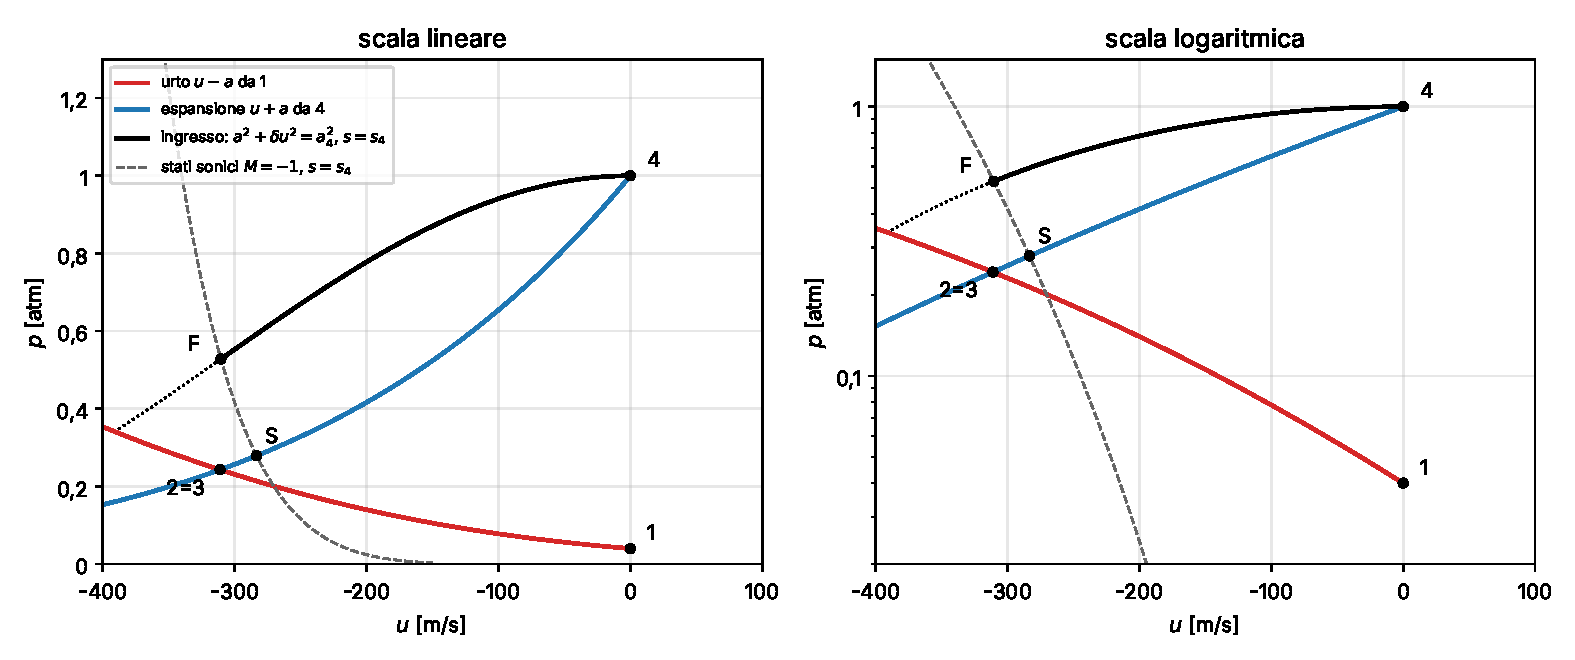
\includegraphics[width=\textwidth]{pu.pdf}
  \caption{Piano $p$--$u$ in scala lineare e logaritmica: curva d'urto da 1, curva d'espansione da 4, curva degli
  stati d'ingresso (nero; punteggiata oltre $M=-1$, non ammessa) e luogo degli stati sonici con $s=s_4$.}
  \label{fig:pu}
\end{figure}
\textbf{Piano $p$--$u$} (fig.~\ref{fig:pu}). L'incrocio fra la curva d'urto uscente da 1 e quella d'espansione
entrante in 4 è lo stato 2=3: le impedenze dei due gas sono molto diverse ($\rho_1a_1\approx29$ contro
$\rho_4a_4\approx417$ kg/(m$^2$s)), e infatti la curva d'urto è molto più piatta, ma il contatto risulta nullo,
cosa che il piano $p$--$u$ da solo non mostra. La curva degli stati d'ingresso parte da 4 con tangente orizzontale
(la pressione scende con $u^2$), mentre la curva d'espansione ha pendenza $\rho_4a_4$: è la ragione per cui la
riflessa è una compressione. Il luogo sonico passa per S (sonico nel ventaglio) e per F (sonico stazionario): F
ha pressione quasi doppia di S perché il gas vi arriva con l'entalpia totale dell'ambiente, mentre l'espansione
instazionaria gliel'ha in parte sottratta. Le pressioni vanno da 0,04 a 1 atm: la scala lineare mostra le distanze
reali fra gli stati (2, 3, S, F sono vicini), quella logaritmica separa bene lo stato 1 e il ramo d'urto.

\begin{figure}[H]
  \centering
  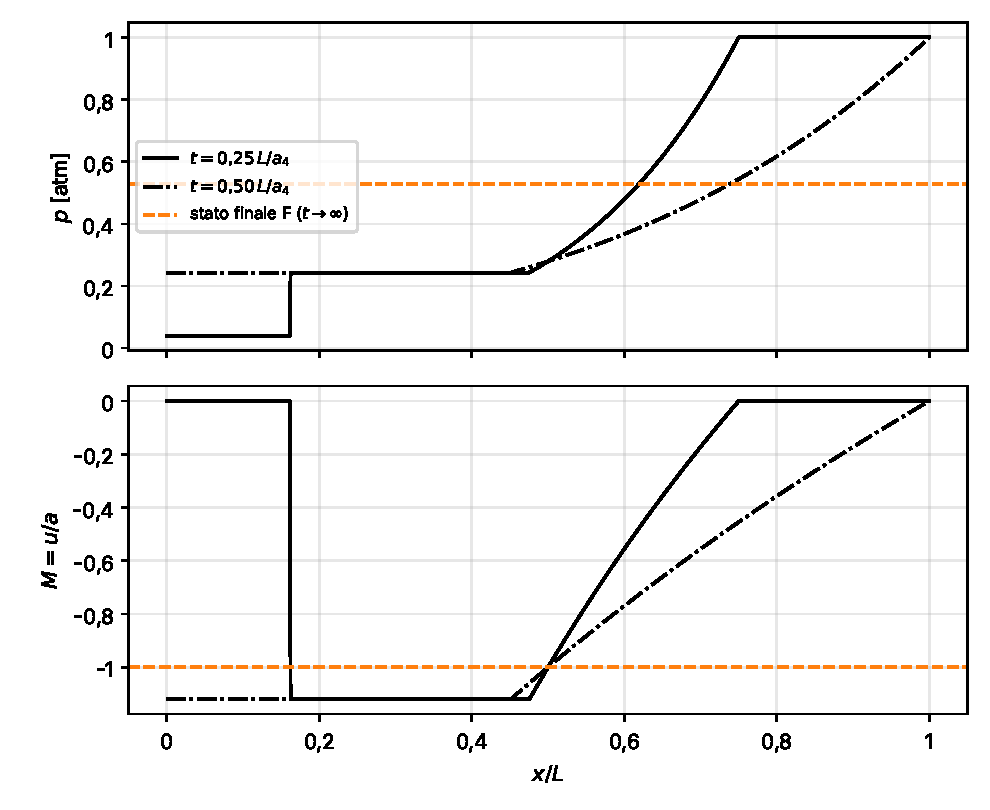
\includegraphics[width=0.72\textwidth]{profili.pdf}
  \caption{Pressione e Mach lungo il condotto a $t=0{,}25\,\tau$ e $t=0{,}5\,\tau$ (esatti) e nello stato finale.}
  \label{fig:profili}
\end{figure}
\textbf{Profili} (fig.~\ref{fig:profili}). A $0{,}25\,\tau$ si vedono il salto d'urto da \num{0.04} a
\SI{0.243}{atm}, il plateau 2--3 senza traccia del contatto e il ventaglio fino a \SI{1}{atm}. A $0{,}5\,\tau$ l'urto è
uscito e il ventaglio occupa tutta la metà destra; il Mach passa per $-1$ esattamente in $x=L/2$. La retta
tratteggiata è lo stato finale: rispetto a $0{,}5\,\tau$ il condotto, a sinistra, deve ancora ricomprimersi (da
\num{0.243} a \SI{0.528}{atm}) e, a destra, espandersi da 1 a \SI{0.528}{atm}.

%==============================================================================
\section{Discussione fisica}
\begin{itemize}
\item \textbf{Contatto nullo.} I dati sono tali che l'urto porta il gas del serbatoio, freddo (\SI{98}{K}),
  esattamente all'entropia dell'ambiente: dopo l'uscita dell'urto il condotto contiene un solo gas omoentropico e il
  transitorio è governato dai soli invarianti di Riemann. Con un serbatoio più caldo o più freddo il contatto
  sarebbe un'onda di entropia che si scarica nel serbatoio a \SI{311}{m/s}, senza cambiare la struttura del resto.
\item \textbf{Grandezze totali nell'instazionario.} Lo stato 3 viene dall'aria ambiente in quiete
  ($p_0=\SI{1}{atm}$, $T_0=\SI{287.7}{K}$) ma ha $p_0=\SI{0.53}{atm}$ e $T_0=\SI{240}{K}$: l'espansione
  instazionaria toglie entalpia totale. Solo a regime, nello stato F, le grandezze totali tornano quelle
  dell'ambiente. È il motivo per cui non si possono usare $p_0$, $h_0$ costanti nel transitorio.
\item \textbf{Condizione d'ingresso.} Imporre all'ingresso la pressione statica ambiente sarebbe sbagliato: la
  riflessa riporterebbe $p$ a \SI{1}{atm} e il gas entrerebbe senza perdere pressione statica, cioè con entalpia
  totale maggiore di quella dell'ambiente. Imponendo $p_0$, $T_0$ la pressione d'ingresso scende fino a quella
  critica, e il condotto si strozza.
\item \textbf{Ruolo del serbatoio.} Dopo $t_0$ il serbatoio non influenza il condotto: l'uscita è sempre
  supersonica o sonica. Lo stato finale è lo stesso per qualunque pressione del serbatoio inferiore a
  \SI{0.528}{atm}. Su tempi lunghi il serbatoio si riempie con portata $\rho^*a^*A$; quando la sua pressione supera
  \SI{0.528}{atm} l'uscita diventa subsonica, si impone $p=p_{\rm serb}$ e parte un nuovo transitorio verso una
  corrente subsonica.
\item \textbf{Durata.} Il transitorio si chiude asintoticamente: le $\upa$ con $R_2$ vicino a $R_2^*$ sono quasi
  ferme e lasciano il condotto lentamente. Con $L=\SI{1}{m}$ ($\tau\approx\SI{2.9}{ms}$) gli scarti da F sono di
  qualche per cento dopo circa 30$\,\tau\approx\SI{0.1}{s}$.
\item \textbf{Limiti del modello.} All'imbocco reale a spigolo vivo il getto entrante si contrae e la sezione
  sonica è la vena contratta: la portata sarebbe minore di $\rho^*a^*A$. Con l'attrito (corrente di Fanno) la
  corrente subsonica accelera verso l'uscita e la sezione sonica si sposta all'uscita. Il getto nel serbatoio e la
  diffrazione dell'urto sono 3D. Nessuno di questi effetti cambia la sequenza delle onde nel condotto.
\end{itemize}

\end{document}
